% Created 2022-02-14 Mon 16:30
% Intended LaTeX compiler: pdflatex
\documentclass[french]{beamer}
\usepackage[utf8]{inputenc}
\usepackage[T1]{fontenc}
\usepackage{graphicx}
\usepackage{longtable}
\usepackage{wrapfig}
\usepackage{rotating}
\usepackage[normalem]{ulem}
\usepackage{amsmath}
\usepackage{amssymb}
\usepackage{capt-of}
\usepackage{hyperref}
\usepackage{minted}
\usepackage[french]{babel}
\usepackage[titles]{tocloft}
\usepackage{listings}
\usepackage[font=scriptsize]{caption}
\usepackage{minted}
\usemintedstyle{xcode}
\definecolor{UBCblue}{rgb}{0.04706, 0.13725, 0.26667} % UBC Blue (primary)
\usecolortheme[named=UBCblue]{structure}
\newminted{sqlite}{fontsize=\footnotesize}
\addtobeamertemplate{footnote}{}{\vspace{2ex}}
\usetheme{default}
\usecolortheme{dolphin}
\usefonttheme{professionalfonts}
\useinnertheme[shadow]{rounded}
\useoutertheme{infolines}
\author{Pierre, Thierno, Bastien, Laurent}
\date{\today}
\title{Créer et utiliser une base de données}
\subtitle{Movie Db}
\titlegraphic{\includegraphics[width=90]{img/iu.png}}
\setbeamerfont{caption}{size=\scriptsize}
\hypersetup{
 pdfauthor={Pierre, Thierno, Bastien, Laurent},
 pdftitle={Créer et utiliser une base de données},
 pdfkeywords={},
 pdfsubject={},
 pdfcreator={Emacs 27.2 (Org mode 9.5.2)}, 
 pdflang={French}}
\begin{document}

\maketitle
\begin{frame}{Outline}
\setcounter{tocdepth}{1}
\tableofcontents
\end{frame}

\section{Milestone 1 : (Modélisation) Analyse fonctionnelle}
\label{sec:orgc2c4664}
\begin{frame}[label={sec:org45241b8},shrink=20]{Données en entrée}
\begin{center}
\begin{tabular}{lrrrrr}
 & count & unique & top & freq & mean\\
\hline
color & 5024 & 2 & Color & 4815 & nan\\
director\_name & 4939 & 2398 & Steven Spielberg & 26 & nan\\
num\_critic\_for\_reviews & 4993 & nan & nan & nan & 140.194\\
duration & 5028 & nan & nan & nan & 107.201\\
director\_facebook\_likes & 4939 & nan & nan & nan & 686.509\\
actor\_3\_facebook\_likes & 5020 & nan & nan & nan & 645.01\\
actor\_2\_name & 5030 & 3032 & Morgan Freeman & 20 & nan\\
actor\_1\_facebook\_likes & 5036 & nan & nan & nan & 6560.05\\
gross & 4159 & nan & nan & nan & 4.84684e+07\\
genres & 5043 & 914 & Drama & 236 & nan\\
actor\_1\_name & 5036 & 2097 & Robert De Niro & 49 & nan\\
movie\_title & 5043 & 4917 & Ben-Hur & 3 & nan\\
num\_voted\_users & 5043 & nan & nan & nan & 83668.2\\
cast\_total\_facebook\_likes & 5043 & nan & nan & nan & 9699.06\\
actor\_3\_name & 5020 & 3521 & John Heard & 8 & nan\\
facenumber\_in\_poster & 5030 & nan & nan & nan & 1.37117\\
plot\_keywords & 4890 & 4760 & based on novel & 4 & nan\\
movie\_imdb\_link & 5043 & 4919 & \url{http://www.imdb.com/title/tt0232500/?ref\_=fn\_tt\_tt\_1} & 3 & nan\\
num\_user\_for\_reviews & 5022 & nan & nan & nan & 272.771\\
language & 5031 & 47 & English & 4704 & nan\\
country & 5038 & 65 & USA & 3807 & nan\\
content\_rating & 4740 & 18 & R & 2118 & nan\\
budget & 4551 & nan & nan & nan & 3.97526e+07\\
title\_year & 4935 & nan & nan & nan & 2002.47\\
actor\_2\_facebook\_likes & 5030 & nan & nan & nan & 1651.75\\
imdb\_score & 5043 & nan & nan & nan & 6.44214\\
aspect\_ratio & 4714 & nan & nan & nan & 2.2204\\
movie\_facebook\_likes & 5043 & nan & nan & nan & 7525.96\\
\end{tabular}
\end{center}
\end{frame}

\begin{frame}[label={sec:orgd9a5857}]{Dictionnaire des données}
\begin{center}
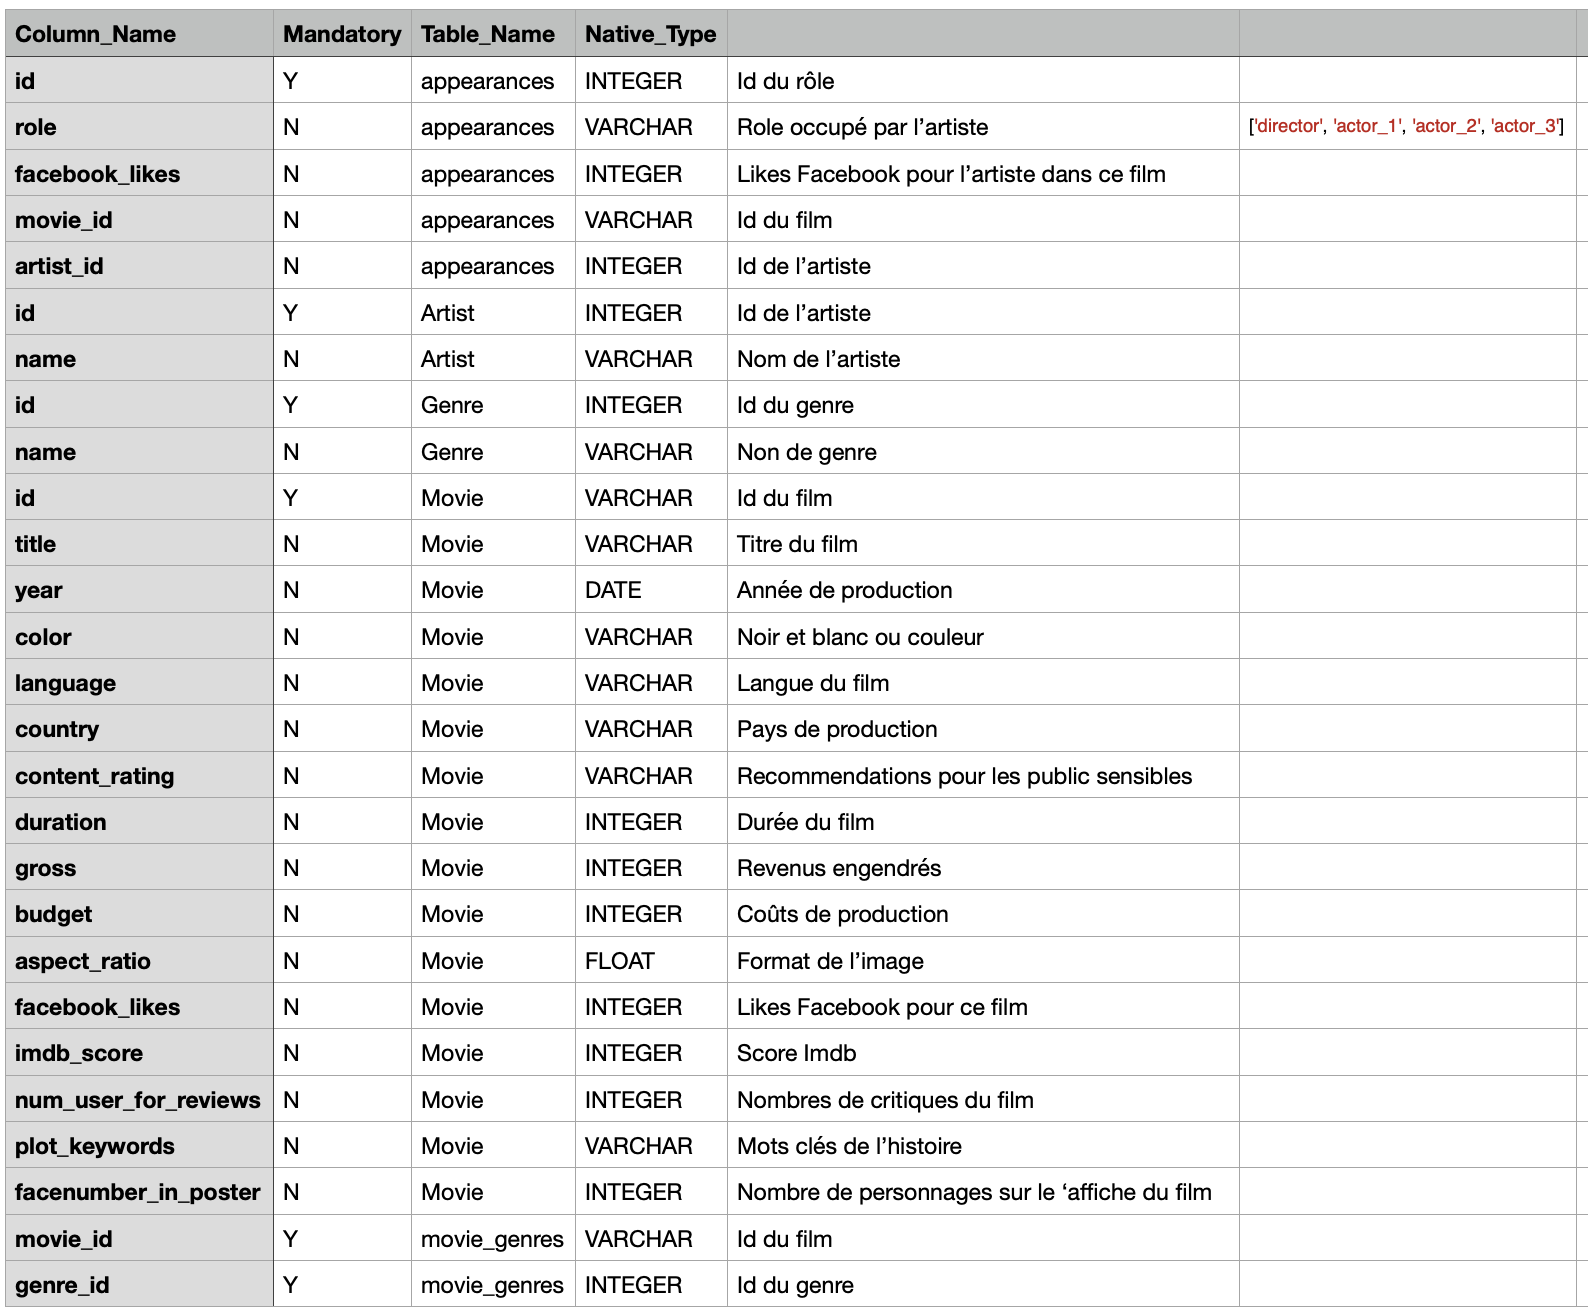
\includegraphics[width=9cm]{./fig/cat.png}
\end{center}
\end{frame}


\section{Milestone 2 : (Modélisation) Modèle conceptuel de données}
\label{sec:org67d6240}
\begin{frame}[label={sec:org7f57c89}]{MCD}
\begin{center}
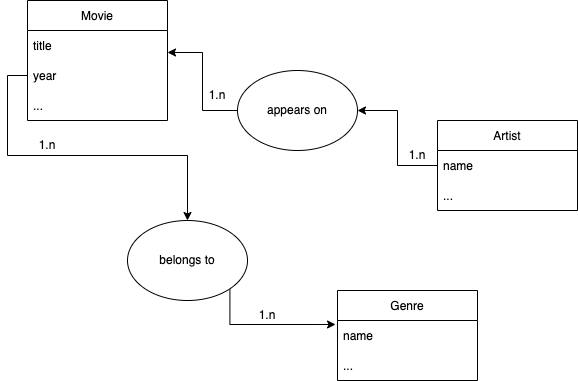
\includegraphics[width=10cm]{./fig/mcd.png}
\end{center}
\end{frame}


\section{Milestone 3 : (Modélisation) Modèle logique de données}
\label{sec:orge866a38}
\begin{frame}[label={sec:org067e138}]{Modèle logique de données}
\begin{center}
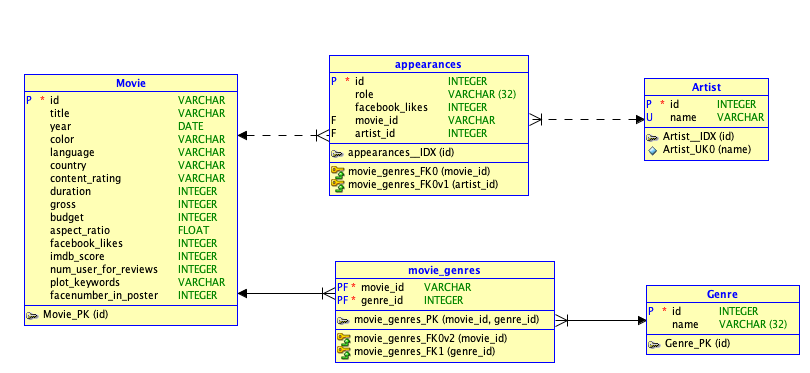
\includegraphics[width=10cm]{./fig/umldb.png}
\end{center}
\end{frame}


\section{Milestone 4 : (Implémentation) Création de la base}
\label{sec:org42e5e79}
\begin{frame}[label={sec:org61a25d6},fragile,shrink=5]{Création de la base de données (SQLAlchemy)}
 \begin{minted}[frame=lines,fontsize=\scriptsize,linenos]{python}
class Movie(Base):
    __tablename__ = 'Movie'
    id = Column(String, primary_key=True, nullable=False) 
    title = Column(String)
    year = Column(Date)
    color = Column(String)
    language = Column(String)
    country = Column(String)
    content_rating = Column(String)
    duration = Column(Integer)
    gross = Column(Integer)
    budget = Column(Integer)
    aspect_ratio = Column(Float)
    facebook_likes = Column(Integer)
    imdb_score = Column(Integer)
    num_user_for_reviews = Column(Integer)
    plot_keywords = Column(String)
    facenumber_in_poster = Column(Integer)
    genres = relationship('Genre', secondary = 'movie_genres', back_populates="movies")
    cast = relationship('Artist', secondary = 'appearances', back_populates="movies")
\end{minted}
\end{frame}

\begin{frame}[label={sec:org648933e},fragile]{Création de la base de données (SQL)}
 \begin{minted}[frame=lines,fontsize=\scriptsize,linenos]{sql}
CREATE TABLE appearances (
	id INTEGER NOT NULL PRIMARY KEY AUTOINCREMENT, 
	role VARCHAR(32), 
	facebook_likes INTEGER, 
	movie_id VARCHAR, 
	artist_id INTEGER, 
	FOREIGN KEY(movie_id) REFERENCES "Movie" (id), 
	FOREIGN KEY(artist_id) REFERENCES "Artist" (id)
)
;
\end{minted}
\end{frame}

\section{Milestone 5 : (Implémentation) Importation des données}
\label{sec:org09e848e}
\begin{frame}[label={sec:org182091a},fragile]{Chargement des donneés}
 \begin{itemize}
\item Extrait du script d'initialisation et de chargement de la base:
\end{itemize}

\begin{minted}[frame=lines,fontsize=\scriptsize,linenos]{python}
roles = ['director', 'actor_1', 'actor_2', 'actor_3']

for i, row in df.iterrows():
    for role in roles:
        a = eval(f'row.{role}_name')
        q = s.query(Artist).filter(Artist.name==a)
        if s.query(q.exists()).scalar():
            artist_id = q.first().id
        else:
            artist = Artist(**{
                'name': eval(f'row.{role}_name')
            })
            s.add(artist)
            s.commit()
            artist_id = q.first().id
\end{minted}
\end{frame}


\section{Milestone 6 : (Exploitation) Requêtes SQL}
\label{sec:orgec4d481}
\begin{frame}[label={sec:org01f8d3b},fragile]{le top 10 des films les plus rentables}
 \begin{minted}[frame=lines,fontsize=\scriptsize,linenos]{sql}
SELECT title,gross-budget FROM Movie ORDER BY gross-budget DESC LIMIT 10
\end{minted}

\begin{center}
\begin{tabular}{lr}
title & gross-budget\\
\hline
Avatar  & 523505847\\
Jurassic World  & 502177271\\
Titanic  & 458672302\\
Star Wars: Episode IV - A New Hope  & 449935665\\
E.T. the Extra-Terrestrial  & 424449459\\
The Lion King  & 377783777\\
Star Wars: Episode I - The Phantom Menace  & 359544677\\
The Dark Knight  & 348316061\\
The Hunger Games  & 329999255\\
Deadpool  & 305024263\\
\end{tabular}
\end{center}
\end{frame}


\begin{frame}[label={sec:org4ff9b60},fragile]{le top 10 des films les moins rentables}
 \begin{minted}[frame=lines,fontsize=\scriptsize,linenos]{sql}
SELECT title,gross-budget FROM Movie ORDER BY gross-budget ASC LIMIT 10
\end{minted}

\begin{center}
\begin{tabular}{lr}
The Host  & -12213298588\\
Lady Vengeance  & -4199788333\\
Fateless  & -2499804112\\
Princess Mononoke  & -2397701809\\
Steamboy  & -2127109510\\
Akira  & -1099560838\\
Godzilla 2000  & -989962610\\
Tango  & -698312689\\
Kabhi Alvida Naa Kehna  & -696724557\\
Red Cliff  & -553005191\\
\end{tabular}
\end{center}
\end{frame}


\begin{frame}[label={sec:orgbcfb3f1},fragile,shrink=5]{les réalisateurs qui ont fait le plus de films}
 \begin{minted}[frame=lines,fontsize=\scriptsize,linenos]{sql}
SELECT
a.name, COUNT(*)
FROM
Artist a
INNER JOIN
(Movie m INNER JOIN appearances p ON m.id = p.movie_id) ON a.id = p.artist_id
WHERE role='director'
GROUP BY a.name
ORDER BY COUNT(*) DESC LIMIT 10;
\end{minted}

\begin{center}
\begin{tabular}{lr}
Steven Spielberg & 26\\
Woody Allen & 22\\
Martin Scorsese & 20\\
Clint Eastwood & 20\\
Spike Lee & 16\\
Ridley Scott & 15\\
Renny Harlin & 15\\
Steven Soderbergh & 14\\
Oliver Stone & 14\\
Ron Howard & 13\\
\end{tabular}
\end{center}
\end{frame}

\begin{frame}[label={sec:org3efeda2},fragile]{l'acteur qui a joué dans le plus de films}
 \begin{minted}[frame=lines,fontsize=\scriptsize,linenos]{sql}
SELECT
a.name, COUNT(*)
FROM
Artist a
INNER JOIN
(Movie m INNER JOIN appearances p ON m.id = p.movie_id) ON a.id = p.artist_id
WHERE role='actor_1' OR role='actor_2' OR role='actor_3'
GROUP BY a.name
ORDER BY COUNT(*) DESC LIMIT 1;
\end{minted}

\begin{center}
\begin{tabular}{lr}
Robert De Niro & 51\\
\end{tabular}
\end{center}
\end{frame}


\begin{frame}[label={sec:orgfaabb1c},fragile]{le nombre de films avec "love" dans les mots clés}
 \begin{minted}[frame=lines,fontsize=\scriptsize,linenos]{sql}
SELECT COUNT(*) From movie WHERE plot_keywords LIKE '% love,%'
\end{minted}

\begin{verbatim}
156
\end{verbatim}
\end{frame}

\begin{frame}[label={sec:org859b5d7},fragile]{le nombre de films français}
 \begin{minted}[frame=lines,fontsize=\scriptsize,linenos]{sql}
SELECT COUNT(*) From movie WHERE language = 'French'
\end{minted}

\begin{verbatim}
64
\end{verbatim}
\end{frame}


\begin{frame}[label={sec:orge155738},fragile]{le réalisateur avec au moins 10 films qui obtient la meilleure moyenne (note imdb)}
 \begin{minted}[frame=lines,fontsize=\scriptsize,linenos]{sql}
SELECT a.name, AVG(m.imdb_score), COUNT(*)
FROM movie m INNER JOIN appearances p
ON m.id = p.movie_id INNER JOIN artist a
ON p.artist_id = a.id WHERE p.role='director'
GROUP BY a.name HAVING COUNT(m.id) > 9
ORDER BY AVG(m.imdb_score) DESC LIMIT 1
\end{minted}

\begin{center}
\begin{tabular}{lrr}
David Fincher & 7.75 & 10\\
\end{tabular}
\end{center}
\end{frame}


\section{Bibliography}
\label{sec:org04ca828}
\begin{frame}[label={sec:org4e90d95}]{References}
\begin{itemize}
\item \url{https://github.com/lsiksous/recsys}
\end{itemize}

\bibliographystyle{unsrt}
\bibliography{recsys}
\end{frame}
\end{document}